\documentclass[a4paper,twoside]{report}
\usepackage[utf8]{inputenc}
% \usepackage[a4paper, width=150mm, top=25mm, bottom=25mm, bindingoffset=6mm]{geometry}
\usepackage{fancyhdr}
\pagestyle{fancy}
 \fancyhead{}
 \fancyhead[LO,LE]{\leftmark}
 \fancyfoot{}
 \fancyfoot[CO,CE]{\thepage}
 \renewcommand{\headrulewidth}{0.2pt}
 \renewcommand{\footrulewidth}{0.2pt}
 \setlength{\headheight}{14.5pt}


% \usepackage{epsfig,epic,eepic,units}
\usepackage{hyperref} %allows to add hyperlinks and cross reference in-text
\usepackage{textcomp} %this is for symbols such as copyright etc
\usepackage{url} %for adding urls obvs so they appear always in one line without breaks
\usepackage{longtable} %allows you to make tables of two or more pages
\usepackage{mathrsfs} %maths fonts, might not need
\usepackage{array} %extends array and tabular environments
\usepackage{multirow} %for tables again
\usepackage{bigstrut} %tables
\usepackage{amssymb} %adding arrows tbh for chemistry you can just use chemmacros \begin{reaction} environment
\usepackage{amsmath} %for writing maths
\usepackage{adjustbox}%supplement to graphics package
\usepackage{graphicx}
\usepackage{lscape} %allows to add certain pages in landscape
\usepackage[nottoc]{tocbibind} %this adds bibliography to your ToC
\usepackage{textgreek} %for upright greek letters
\usepackage{siunitx} %you can declare the units you want as necessary read documentation
\usepackage{biblatex}
\usepackage[
    asymmetric,
    a4paper,
    left=3cm,
    right=2cm,
    top=2.75cm,
    bottom=3cm,
    footskip=0cm,
    twoside]{geometry}

    \usepackage{tikz}
\usetikzlibrary {automata,positioning}

% add commands
\usepackage{commands}

\addbibresource{refs.bib}

\begin{document}
\sloppy

\begin{titlepage}
  \begin{center}
    % Logos aligned horizontally
    \begin{minipage}{0.45\textwidth}
      \centering
      
\includegraphics[width=0.8\linewidth]{logo-unilim.png}
    \end{minipage}
    \hfill
    \begin{minipage}{0.45\textwidth}
      \centering
      
\includegraphics[width=0.8\linewidth]{logo-unilim.png}
    \end{minipage}

    \vspace{1cm}

    \Large
    University of Limoges\\
    \vspace{0.5cm}

    \large
    \textbf{Internship report}\\
    Master 2 ACSYON

    \vspace{1.5cm}

    % Divider before the title
    \noindent\rule{\textwidth}{0.4pt}
    \vspace{0.5cm}

    \Large
    \textbf{Title}

    \vspace{0.5cm}
    % Divider after the title
    \noindent\rule{\textwidth}{0.4pt}

    \vfill

    CHAU Dang Minh

    \vfill

    \Large
    \textbf{Supervisor:}

    \vfill

    \large
    Limoges, September 2025

  \end{center}
\end{titlepage}
 %title file for the front page
\renewcommand*\contentsname{Table of Contents} %this is to have the correct heading on the ToC
\tableofcontents %make table of contents

\include{chapters/section-types
}
\chapter{Open Automata}
\section{Open Automaton for Sliding Window Protocols}

Description

\begin{itemize}
  \item If the frame to send does not lie outside of the window, send this frame
  \item If the correct ACK is send, increase the window index by 1 and take modulo $N$
\end{itemize}

We use a fix window size $N$ and a limit waiting time $T > 0$. Variables are
\begin{itemize}
  \item The window index $w$
  \item The current frame's index $i$
  \item The waited time $t$
\end{itemize}

The Sender can dispatch \texttt{getFrame}, \texttt{send}, \texttt{wait}, \texttt{resend}. Meanwhile, the Receiver can dispatch \texttt{ack} when a frame is delivered correctly. Therefore, the transitions are as follows

$$\begin{aligned}
    s_1 & = \dfrac{\{\text{Sender}\mapsto \texttt{getFrame}(i)\}(\text{True})\{\}}{q_0\xrightarrow{\tau}q_0}                                \\
    s_2 & = \dfrac{\{\text{Sender}\mapsto \texttt{send}(M[i])\}((i+1)\% N \neq w)\{i:= (i + 1)\%N\}}{q_0\xrightarrow{\text{frameSent}}q_0}  \\
    s_3 & = \dfrac{\{\text{Sender}\mapsto \texttt{wait}\}((i+1)\% N = w \wedge t < T)\{t:= t + 1\}}{q_0\xrightarrow{\tau}q_0}               \\
    s_4 & = \dfrac{\{\text{Sender}\mapsto \texttt{resend}(M[w])\}(t = T)\{t:= 0\}}{q_0\xrightarrow{\text{frameResent}}q_0}                  \\
    t_1 & = \dfrac{\{\text{Receiver}\mapsto \texttt{ack}(M[w])\}(w \neq i)\{w:= (w + 1)\%N; t:= 0\}}{q_0\xrightarrow{\text{frameAcked}}q_0} \\
  \end{aligned}
$$

\begin{center}
  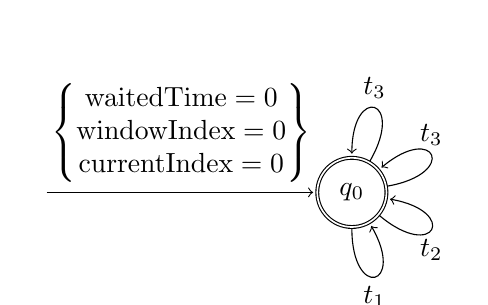
\begin{tikzpicture}[shorten >=1pt,node distance=2cm,on grid,auto]

    \node[]               (init_assign)
    {};
    \node[state, accepting] (q_0) [right=4cm of init_assign] {$q_0$};


    \path[->]
    (init_assign) edge node {$\begin{Bmatrix}
            \text{waitedTime} = 0   \\
            \text{windowIndex} = 0  \\
            \text{currentIndex} = 0 \\
          \end{Bmatrix}$} (q_0)
    (q_0) edge [loop, in=-60, out=-90, looseness=10] node[pos=0.5, anchor=north] {$t_1$} (q_0)
    (q_0) edge [loop, in=-10, out=-40, looseness=10] node[pos=0.5, anchor=north] {$t_2$} (q_0)
    (q_0) edge [loop, in=40, out=10, looseness=10] node[pos=0.5, anchor=south] {$t_3$} (q_0)
    (q_0) edge [loop, in=90, out=60, looseness=10] node[pos=0.5, anchor=south] {$t_3$} (q_0)
    ;

  \end{tikzpicture}
\end{center}

\printbibliography

\end{document}
